\documentclass[conference]{IEEEtran}
\IEEEoverridecommandlockouts
\usepackage{cite}
\usepackage{amsmath,amssymb}
\usepackage{graphicx}
\usepackage{booktabs}
\usepackage{array}
\usepackage[hidelinks]{hyperref}
\usepackage{xcolor}
\hypersetup{pdfauthor={Shubhodeep Chatterjee}, pdftitle={Per-Disease Cytogenetic Progression Models from the Mitelman Database: Co-occurrence, Conjunctive Bayesian Networks and Mutual Hazard Networks}}
\graphicspath{{figures/}}
\begin{document}
\title{Per-Disease Cytogenetic Progression Models from the Mitelman Database: Co-occurrence, Conjunctive Bayesian Networks and Mutual Hazard Networks}
\author{\IEEEauthorblockN{Shubhodeep Chatterjee}\IEEEauthorblockA{Independent research \\ github.com/shubhodeepcx/MitelmanProgression}}
\maketitle
\begin{abstract}
We built per-disease models of cytogenetic progression for seven haematological malignancies from 52,054 non-duplicate karyotypes in the Mitelman Database. Clone structure was parsed from ISCN notation, events were frozen per disease by a power calculation, and three existing methods were fitted to the same data: a co-occurrence baseline with a count-preserving permutation null, a conjunctive Bayesian network (CBN) and a Mutual Hazard Network (MHN). Five diseases had at least 200 cases with a within-patient clone order; APL and myeloma were limited to the baseline. The MHN fitted held-out data better than independence and than the CBN in every disease, its interactions were stable under the bootstrap, and they held in unselected series and in post-2000 publications. Simulation recovery was adequate in AML, ALL and CLL and failed in MDS and CML. The MHN's event orders, however, agreed with the within-patient clone orders only in CML; in the other diseases they agreed at about chance level, because events that are often seen alone, such as trisomy 8, are placed first. The sparse CBN posets agreed with the clone orders in 22 of 23 testable cases. The supported conclusions are therefore the interaction structure from the MHN and the orders backed by the clone data and the CBN, not the MHN's orders on their own. Code, event tables and figures are released.
\end{abstract}
\begin{IEEEkeywords}
Cancer cytogenetics, karyotype, ISCN, Mitelman Database, tumour progression, Mutual Hazard Networks, conjunctive Bayesian networks, haematological malignancy
\end{IEEEkeywords}

\section{Introduction}
Chromosomal aberrations in haematological malignancies are not acquired at once. A founding rearrangement such as t(8;21) or t(9;22) is followed by secondary gains and losses, and the secondary changes that accompany a given founder are characteristic rather than random \cite{johansson2002,grimwade2010}. Knowing the usual order of events, and which events promote or suppress one another, is a description of clonal evolution that complements outcome-based classifications.

The Mitelman Database of Chromosome Aberrations and Gene Fusions in Cancer \cite{mitelman} collects every published cancer karyotype in ISCN notation \cite{iscn2020}. Two kinds of ordering signal are available in it. Within a patient, a karyotype that lists a stemline and sidelines states which aberrations are shared by all abnormal cells and which were added later. Across patients, the joint distribution of events carries the information that cancer progression models such as oncogenetic trees \cite{desper1999}, conjunctive Bayesian networks (CBN) \cite{beerenwinkel2007,gerstung2009} and Mutual Hazard Networks (MHN) \cite{schill2020} turn into an order. Earlier multivariate analyses of Mitelman data described karyotypic pathways in solid tumours \cite{hoglund2001}; here the aim is a per-disease model for the haematological malignancies with explicit validation.

\textbf{Claim and scope.} For each disease with enough multi-clone cases, the study asks which pairwise orderings and interactions between recurrent cytogenetic events are supported by the data, with an uncertainty estimate for each, and which are not. It fits existing methods only, and it makes no clinical claims: the orders describe the published case mix.

The contributions are: (i) an open pipeline with one entry point, from the Mitelman bulk files to per-disease event tables, models, validation tables and figures; (ii) a released tidy event table with inferred clone trees; (iii) a co-occurrence baseline, a CBN and an MHN fitted per disease on the same data; and (iv) six validation checks with pre-specified pass thresholds and stop rules.

\section{Data and Biases}
\subsection{Source and cohorts}
The Mitelman bulk download (md5 434cf3759ba633e4d9d99e2bb8208283) holds 81,148 cases from 12,342 references. Diseases were assigned from morphology codes: acute myeloid leukaemia (AML, excluding acute promyelocytic leukaemia), acute promyelocytic leukaemia (APL, morphology code or t(15;17) in a myeloid case), myelodysplastic neoplasms (MDS), chronic myeloid leukaemia (CML), acute lymphoblastic leukaemia (ALL), chronic lymphocytic leukaemia (CLL) and multiple myeloma (MM). After removing likely duplicates, 52,054 cases remain (Table~\ref{tab:data}).

\begin{table}[!t]
\centering
\caption{Cohorts, vocabulary and ordering yield (non-duplicate cases). N: minimum event count from the power calculation. Clone order: cases with at least one parent-to-child event pair, of which Unsel. are from unselected series.}
\label{tab:data}
\footnotesize
\setlength{\tabcolsep}{3pt}
\begin{tabular}{lrrrrrl}
\toprule
\textbf{Disease} & \textbf{Cases} & \textbf{N} & \textbf{Events} & \textbf{Clone order} & \textbf{Unsel.} & \textbf{Models} \\
\midrule
AML & 20,753 & 201 & 20 & 1,471 & 567 & all three \\
APL & 2,341 & 196 & 2 & 64 & 31 & baseline \\
MDS & 5,734 & 200 & 13 & 403 & 112 & all three \\
CML & 4,819 & 199 & 9 & 251 & 156 & all three \\
ALL & 12,842 & 201 & 20 & 609 & 136 & all three \\
CLL & 3,469 & 198 & 6 & 226 & 113 & all three \\
MM & 2,096 & 195 & 16 & 55 & 34 & baseline \\
\bottomrule
\end{tabular}
\end{table}
\subsection{Biases}
\begin{itemize}
\item \textbf{Publication and selection bias.} Mitelman marks each series as Unselected (consecutive cases) or Selected (published for an unusual feature). Selected series over-represent rare rearrangements: in AML, for example, t(8;21) and KMT2A rearrangements are about 1.3 to 1.4 times as frequent in Selected as in Unselected series. Every MHN was refitted on Unselected cases only.
\item \textbf{Era.} Banding resolution and reporting practice changed over five decades; MHNs were refitted on cases published from 2000.
\item \textbf{Duplicate patients.} There is no usable patient identifier. Cases from different references with the same disease, sex, age and an identical karyotype string seen at most three times in the database were treated as one patient; 245 cases were flagged and excluded.
\item \textbf{Cryptic lesions.} Karyotyping misses cryptic rearrangements (for example t(12;21) in ALL) and small copy-number changes, so frequencies understate them.
\item \textbf{Cross-sectional sampling.} Most cases contribute one investigation; ordering is inferred from patterns across cases plus the clone structure within cases.
\end{itemize}
\section{Method}
\subsection{Parsing clones and building events}
Each karyotype is split into clones, and each clone into aberration tokens. The idem shorthand is expanded to the stemline's aberrations (and multiplied for idemx2 polyploid sidelines), opposite numerical changes cancel, sex-chromosome complements and uncounted markers are ignored. A clone's parent is the largest abnormal clone in the same investigation whose aberrations are a proper subset of its own (ties go to the earlier-listed clone); every event in a parent precedes every event the child adds. Copy-number events are the union of what the ISCN text states and arm-level calls from the CytoConverter \cite{cytoconverter} segments shipped with Mitelman, computed relative to each clone's own baseline ploidy ($\geq$ 50\% of an arm, $\geq$ 90\% of a chromosome). The complex-karyotype flag follows ELN 2022 \cite{dohner2022}.

The parser was tested on 50 karyotypes drawn by stratified sampling (single clone, idem sidelines, three or more clones, idemx2, unrelated clones, constitutional and uncertain aberrations, KMT2A variants, CML and MDS multi-clone cases) and annotated by hand in an independent review pass. The parser reproduces every annotated feature set, parent and ordered pair; the full suite has 80 tests.

\subsection{Event vocabulary and power}
Candidate events per disease were listed from the cytogenetics literature before any ordering result was looked at. An event enters the vocabulary if at least N non-duplicate cases carry it, where N is the smallest count giving 80\% power for Fisher's exact test at a Bonferroni level of 0.05/190 (20 events) to detect both an odds ratio of 3 and one of 0.2 against a partner of 10\% frequency. This gives N $\approx$ 200 in every disease. At most 20 events are kept per disease and defining events are always kept. The vocabulary was then frozen. Count-derived events (complex, high hyperdiploid, hypodiploid) are functions of the others and enter the baseline only.

\subsection{Co-occurrence baseline}
For every event pair, Fisher's exact test is compared with a permutation null that keeps each case's number of events fixed and the event frequencies approximately matched (weighted sampling without replacement through Gumbel top-k draws, weights calibrated by iterative scaling, 1,000 permutations). This removes the busy-karyotype effect, where complex cases make every pair look co-occurring. Both p-value sets are corrected by Benjamini-Hochberg \cite{bh1995}; a pair is significant if both q $<$ 0.05 and both tests agree on the direction.

\subsection{Conjunctive Bayesian network}
A CBN is a partial order on events: an event can occur only after all its parents \cite{beerenwinkel2007}. Hidden genotypes compatible with the poset are generated with per-event probabilities $\theta_{i}$, and each observed bit is flipped with probability $\varepsilon$, as in H-CBN \cite{gerstung2009}. $\theta$ and $\varepsilon$ are fitted by expectation maximisation over the enumerated genotypes, and the poset by greedy BIC search with add, remove and reverse moves. The reference C implementations could not be obtained in the analysis environment, so the published discrete-time model was implemented and checked on simulated posets. Because genotypes are enumerated, the CBN uses the 10 most frequent model events per disease.

\subsection{Mutual Hazard Network}
An MHN \cite{schill2020} models progression as a continuous-time Markov chain on the 2$^n$ event states. With event set x already present, event i occurs at rate

\begin{equation}\lambda_i(x) = \Theta_{ii} \prod_{j \in x} \Theta_{ij},\end{equation}
so log $\Theta_{ij}$ $>$ 0 means event j, once present, promotes event i, and log $\Theta_{ij}$ $<$ 0 means it inhibits it. Tumours are observed at an Exp(1) time. Because every event shares that observation time, events with no interaction are still positively associated in the observed data, so log $\theta$ is relative to this shared-time association, not to independence. The likelihood and its gradient were computed with state-space restriction (only states below an observed state are visited). The reference mhn package returned non-finite scores for states with five or six events in this environment, so the likelihood was reimplemented and checked against the package on smaller states, against a closed form for diagonal $\Theta$ and against finite differences. $\Theta$ is fitted by L-BFGS-B on the mean log-likelihood minus $\lambda$ times a smooth L1 penalty on the off-diagonal entries, with $\lambda$ = c/N and c $\in$ \{0.1, 0.3, 1, 3\} chosen by 2-fold held-out likelihood. Order probabilities P(a before b | both present) come from 20,000 simulated trajectories.

\subsection{Validation and stop rules}
Six checks were specified before the fits: (1) bootstrap stability (25 MHN and 20 CBN refits); (2) held-out likelihood against an independence model; (3) simulation recovery (three data sets drawn from each fitted model at the real sample size and refitted); (4) concordance with a written test set of established relationships; (5) agreement with the within-patient clone orders, which the cross-sectional MHN never sees; and (6) publication-bias and era sensitivity refits. An MHN interaction is an edge if |log $\theta$| $\geq$ 0.5 and stable if it keeps its sign in $\geq$ 80\% of bootstrap refits. Simulation recovery is adequate if mean precision $\geq$ 0.8 and recall $\geq$ 0.5. Stop rules: a disease with fewer than 200 cases with a clone order gets the co-occurrence baseline only; failed simulation recovery is reported as the finding; when fewer than half the edges are stable, only the stable subset is presented.

\section{Results}
\subsection{Co-occurrence baseline}
Table~\ref{tab:cooc} counts the significant pairs. Mutual exclusivity dominates wherever founding rearrangements are in the vocabulary: in AML, t(8;21), inv(16), KMT2A rearrangements and inv(3)/t(3;3) exclude one another and the secondary changes of complex karyotypes, and in ALL the founding translocations exclude the trisomies of high hyperdiploidy. Requiring Fisher's test and the permutation null to agree on the direction mattered: some pairs, 31 of them in ALL, co-occur more often than under independence but less often than busy karyotypes alone would predict, and they are no longer called.

\begin{table}[!t]
\centering
\caption{Pairwise baseline: pairs significant under both Fisher's test and the count-preserving null (BH q $<$ 0.05, same direction).}
\label{tab:cooc}
\footnotesize
\setlength{\tabcolsep}{3pt}
\begin{tabular}{lrrrr}
\toprule
\textbf{Disease} & \textbf{Pairs} & \textbf{Significant} & \textbf{Co-occurring} & \textbf{Exclusive} \\
\midrule
AML & 190 & 141 & 58 & 83 \\
APL & 1 & 0 & 0 & 0 \\
MDS & 78 & 36 & 19 & 17 \\
CML & 36 & 22 & 10 & 12 \\
ALL & 190 & 130 & 47 & 83 \\
CLL & 15 & 9 & 5 & 4 \\
MM & 120 & 51 & 33 & 18 \\
\bottomrule
\end{tabular}
\end{table}
\subsection{Model-free clone orders}
The clone trees give direct within-patient evidence (Table~\ref{tab:cloneorders}). The orders are lopsided and match the established biology: 5q loss precedes 17p loss (96:5) and -7 in AML, t(8;21) precedes -Y and -X, inv(16) precedes +22, t(9;22) precedes the extra Ph and +8 in CML, and 5q loss precedes 17p loss in MDS. Trisomy 8 is a secondary event in nearly every case where it shares a karyotype with a founding change (KMT2A 61:4, inv(16) 44:1).

\begin{table}[!t]
\centering
\caption{Model-free orders: the event pairs most often split between a parent clone and its child (non-duplicate cases), with a two-sided sign test.}
\label{tab:cloneorders}
\footnotesize
\setlength{\tabcolsep}{3pt}
\begin{tabular}{lllr}
\toprule
\textbf{Disease} & \textbf{Order} & \textbf{a$\rightarrow$b : b$\rightarrow$a} & \textbf{p} \\
\midrule
AML & 5q loss $\rightarrow$ 17p loss & 96:5 & 7e-23 \\
 & 5q loss $\rightarrow$ +8 & 96:10 & 9e-19 \\
 & t(8;21) $\rightarrow$ -Y & 75:2 & 4e-20 \\
 & 5q loss $\rightarrow$ -7 & 71:14 & 2e-10 \\
MDS & 5q loss $\rightarrow$ +8 & 51:8 & 9e-09 \\
 & 5q loss $\rightarrow$ -7 & 39:9 & 2e-05 \\
 & 5q loss $\rightarrow$ 18 loss & 28:6 & 2e-04 \\
 & 5q loss $\rightarrow$ +21 & 25:1 & 8e-07 \\
CML & t(9;22) $\rightarrow$ +8 & 121:10 & 2e-25 \\
 & t(9;22) $\rightarrow$ extra Ph & 85:0 & 5e-26 \\
 & t(9;22) $\rightarrow$ +19 & 54:0 & 1e-16 \\
 & 17p loss $\rightarrow$ +8 & 38:8 & 9e-06 \\
ALL & t(9;22) $\rightarrow$ 9p loss & 31:1 & 2e-08 \\
 & +21 $\rightarrow$ 1q gain & 29:4 & 1e-05 \\
 & +6 $\rightarrow$ 1q gain & 28:2 & 9e-07 \\
 & +X $\rightarrow$ 1q gain & 26:1 & 4e-07 \\
CLL & +12 $\rightarrow$ 13q loss & 27:2 & 2e-06 \\
 & 13q loss $\rightarrow$ 11q- & 20:6 & 0.009 \\
 & +12 $\rightarrow$ 11q- & 14:2 & 0.004 \\
 & +12 $\rightarrow$ 17p loss & 10:1 & 0.012 \\
\bottomrule
\end{tabular}
\end{table}
\begin{figure*}[!t]
\centering
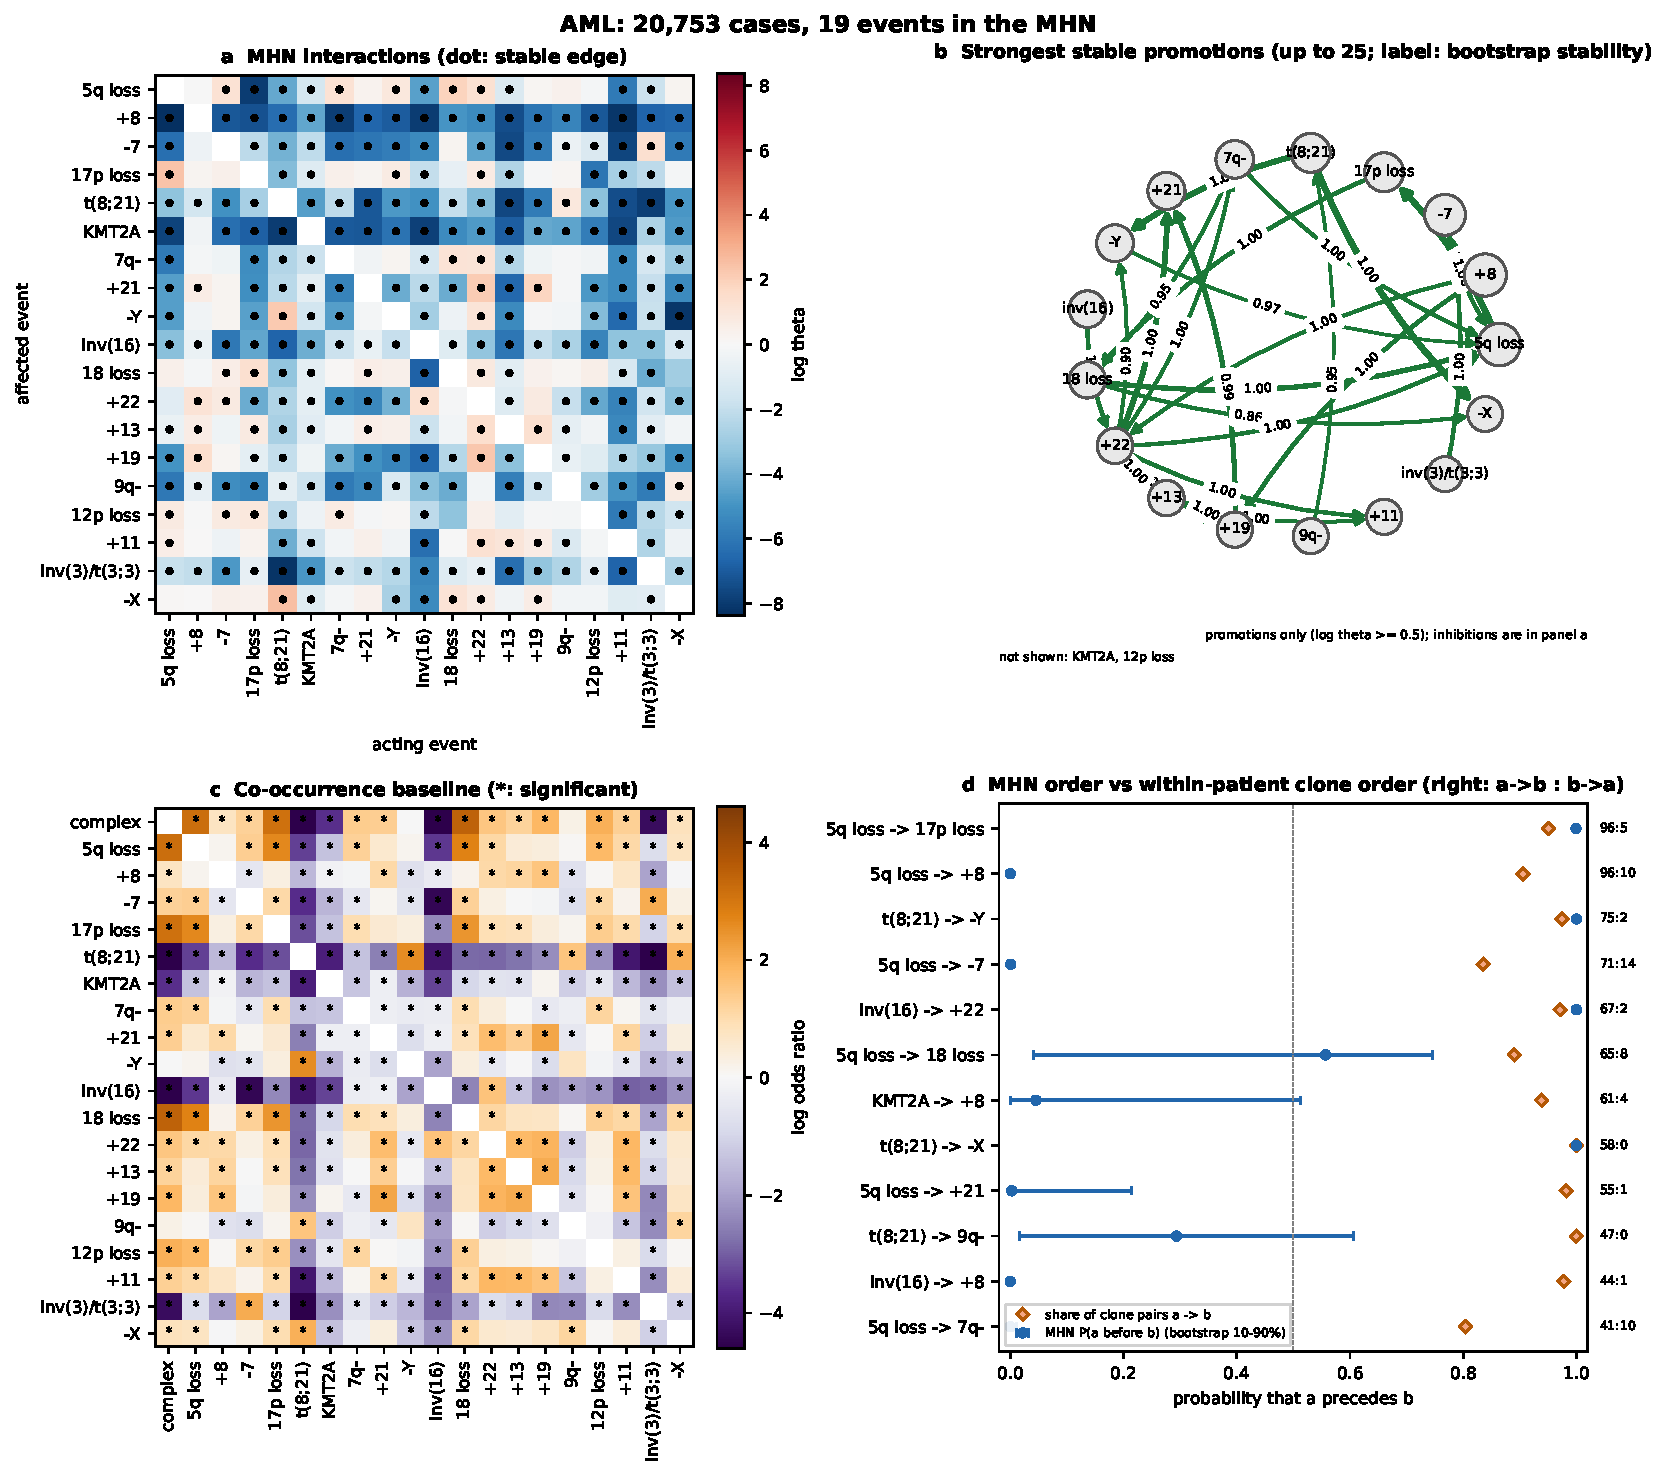
\includegraphics[width=\textwidth]{AML}
\caption{AML. (a) MHN log $\theta$ (row: affected event, column: acting event); dots mark stable edges. (b) Strongest stable promotions; edge labels give bootstrap sign stability. (c) Co-occurrence baseline, log odds ratio; * significant. (d) For the pairs with the most clone evidence, the MHN's P(a before b) with its bootstrap 10-90\% interval (blue) against the share of clone pairs ordered a$\rightarrow$b (orange).}
\label{fig:aml}
\end{figure*}
\begin{figure*}[!t]
\centering
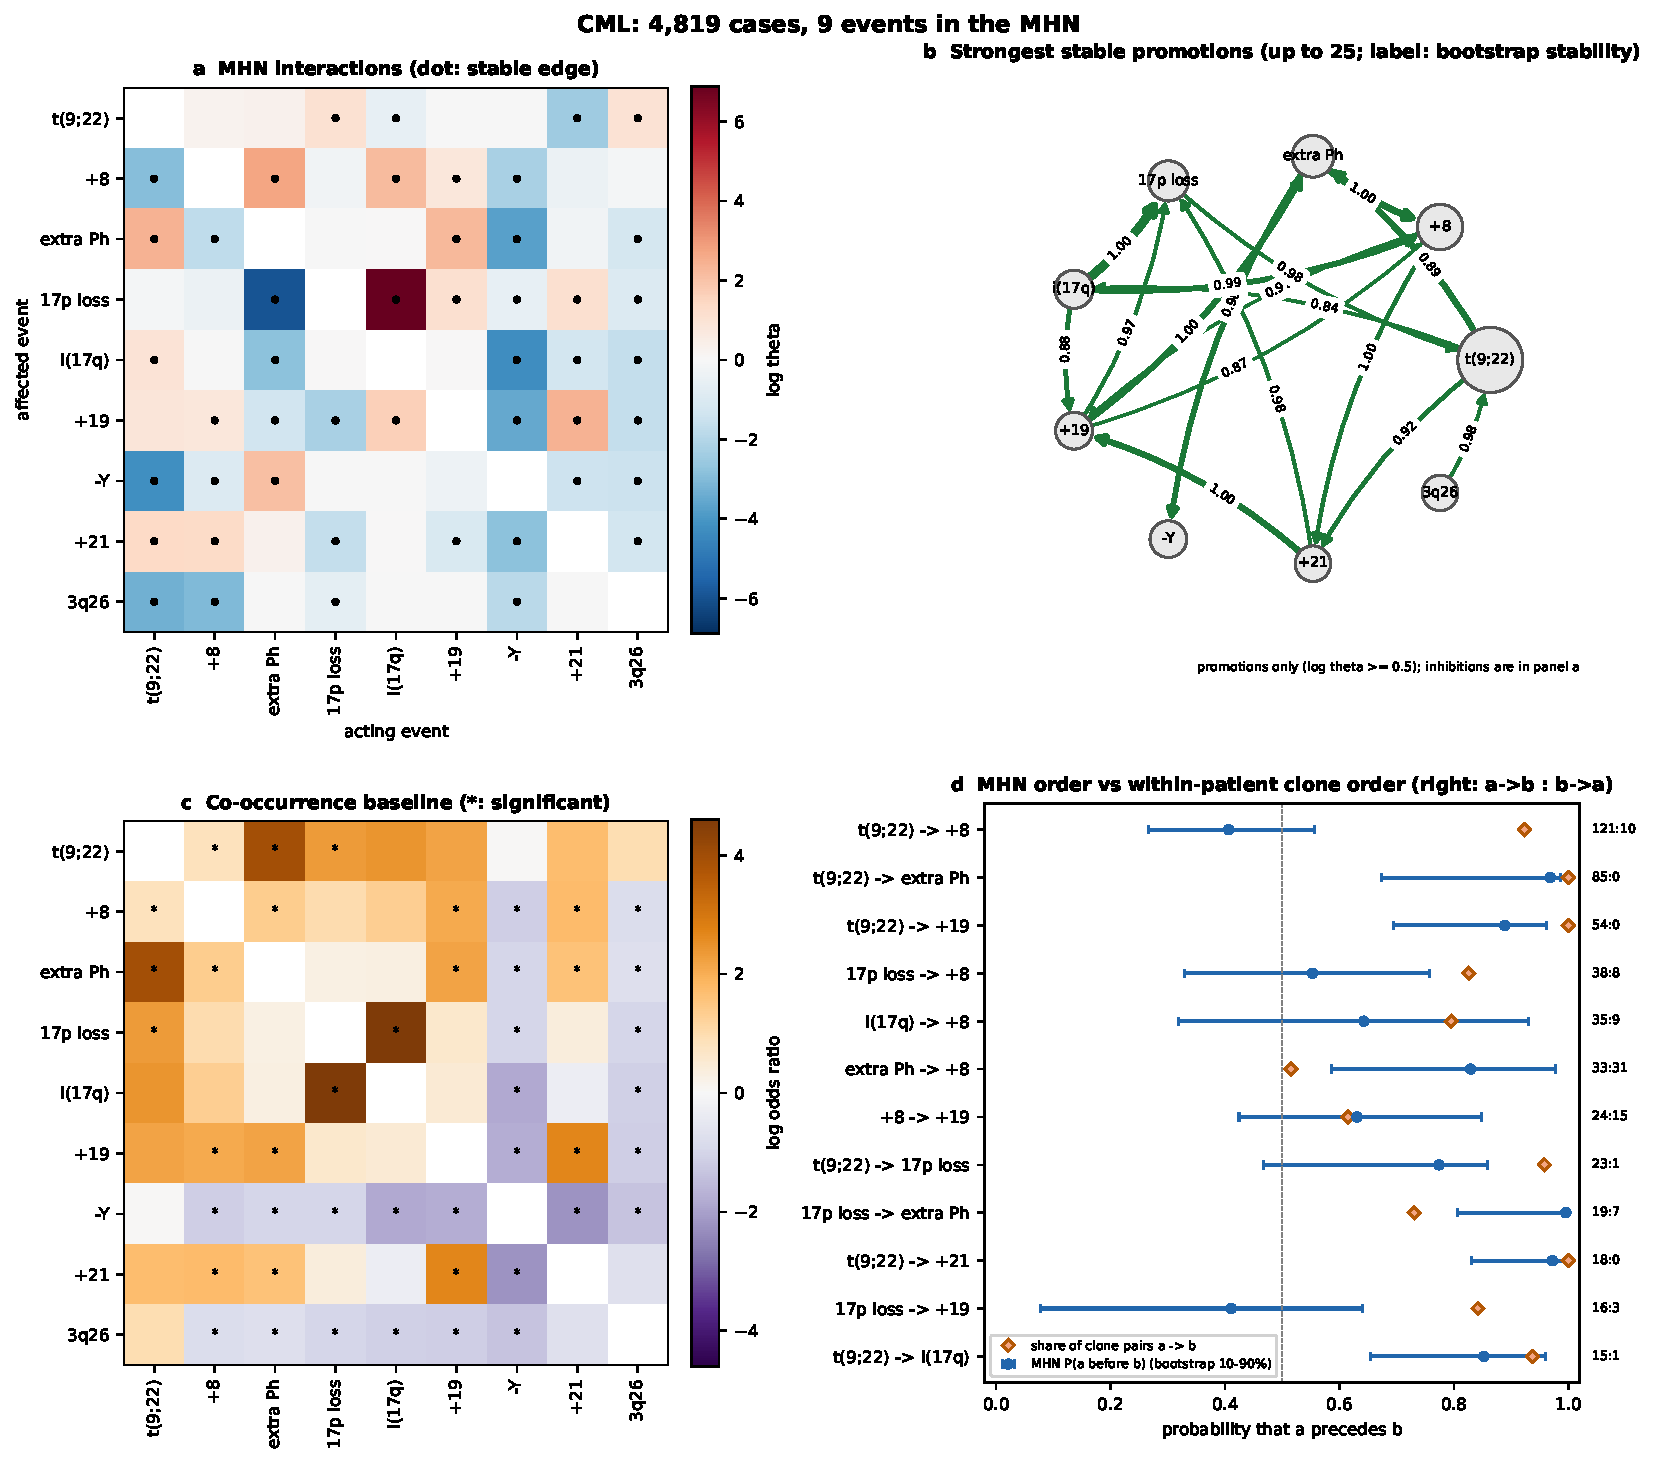
\includegraphics[width=\textwidth]{CML}
\caption{CML, panels as in Fig.~\ref{fig:aml}. Here the MHN's orders and the clone orders agree.}
\label{fig:cml}
\end{figure*}
\begin{figure}[!t]
\centering
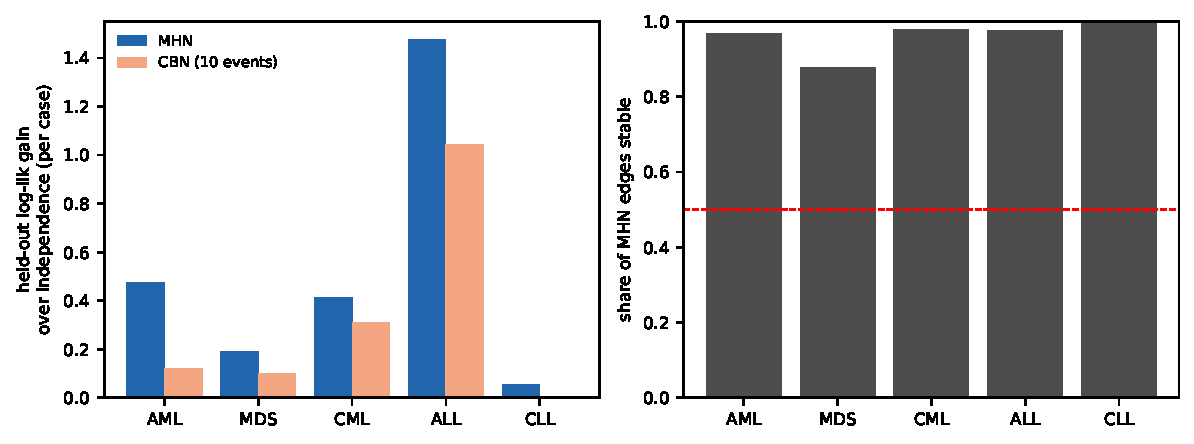
\includegraphics[width=\columnwidth]{overview}
\caption{Held-out log-likelihood gain over independence (MHN on all model events, CBN on ten) and share of stable MHN edges per disease; the dashed line is the 50\% stability rule.}
\label{fig:overview}
\end{figure}
\subsection{Mutual Hazard Networks}
Table~\ref{tab:mhn} summarises the MHN fits. Held-out log-likelihood beat the independence model in all five diseases, by 0.47 nats per case in AML and 1.47 in ALL. Between 88\% and 100\% of edges kept their sign in at least 80\% of bootstrap refits, so every disease passes the stability rule. The refits on unselected series (r = 0.80 to 0.95) and on cases published from 2000 (r = 0.84 to 0.98) reproduce the full-data networks, so publication bias and era do not drive them.

Most interactions are negative. This is expected: log $\theta$ is measured against the positive association that a shared observation time alone produces, so mild raw co-occurrence still carries a negative log $\theta$. In CLL, for example, every interaction except 11q- on 13q loss is negative, yet the fitted model reproduces every observed pairwise odds ratio. The strongest stable promotions are biologically familiar: t(8;21) on -X and -Y, 5q loss on 17p loss, +22 on +19 and +21 in AML; the extra Ph on +8 and +21 on +19 in CML; +21 on the other trisomies of high hyperdiploidy in ALL \cite{moorman2012}; and 18 loss on 17p loss in MDS. Two strong edges are definitional: 17p loss on i(17q) in CML, where the events are nested, and t(1;19) on 1q gain in ALL, where the unbalanced der(19)t(1;19) carries the gain.

Simulation recovery was adequate in AML, ALL and CLL (precision and recall of 0.84 or more) and failed in MDS and CML: refitted networks recovered only 0.56 (MDS) and 0.72 (CML) of their own edges. By the pre-specified rule this failure is the finding for those two diseases: at their sample sizes the MHN's individual edges are not identifiable, even though the networks are stable under resampling.

\begin{table*}[!t]
\centering
\caption{MHN fits and validation. Held-out values are mean log-likelihood per case (2-fold). Stable: bootstrap sign agreement $\geq$ 0.8. Sim P/R: simulation-recovery precision and recall. U and 2000+: correlation of off-diagonal log $\theta$ between the full fit and the refits on unselected series and on cases published from 2000.}
\label{tab:mhn}
\footnotesize
\setlength{\tabcolsep}{3pt}
\begin{tabular}{lrrrrrrrrrr}
\toprule
\textbf{Disease} & \textbf{Events} & \textbf{c} & \textbf{MHN} & \textbf{Indep.} & \textbf{Edges} & \textbf{Stable} & \textbf{Share} & \textbf{Sim P/R} & \textbf{U r} & \textbf{2000+ r} \\
\midrule
AML & 19 & 0.10 & -4.212 & -4.682 & 269 & 264 & 0.98 & 0.88/0.85 & 0.89 & 0.95 \\
MDS & 12 & 0.30 & -3.726 & -3.905 & 90 & 79 & 0.88 & 0.56/0.59 & 0.80 & 0.84 \\
CML & 9 & 1.00 & -2.622 & -3.033 & 42 & 42 & 1.00 & 0.72/0.64 & 0.95 & 0.88 \\
ALL & 18 & 0.30 & -4.271 & -5.744 & 234 & 229 & 0.98 & 0.88/0.88 & 0.84 & 0.95 \\
CLL & 5 & 0.30 & -2.045 & -2.100 & 15 & 15 & 1.00 & 0.90/0.96 & 0.95 & 0.98 \\
\bottomrule
\end{tabular}
\end{table*}
\subsection{Conjunctive Bayesian networks}
The CBNs are sparse (Table~\ref{tab:cbn}). In AML the poset has 5q loss before -7, 7q- and 17p loss, +8 before +21 and t(8;21) before -Y; in CML t(9;22) precedes the extra Ph, 17p loss, +19 and 3q26 rearrangements; in ALL +21 precedes the other hyperdiploid trisomies; in CLL 13q loss precedes 11q- and 17p loss. Simulation recovery was perfect in every disease and the noise rate $\varepsilon$ stayed between 0.016 and 0.098. On the same ten events the MHN fitted held-out data better than the CBN in every disease, so the CBN's hard precedence constraints cost likelihood.

\begin{table*}[!t]
\centering
\caption{CBN on the 10 most frequent model events per disease: noise $\varepsilon$, held-out log-likelihood per case against an MHN and an independence model on the same events, simulation recovery, and the cover relations of the fitted poset with their bootstrap frequency.}
\label{tab:cbn}
\footnotesize
\setlength{\tabcolsep}{3pt}
\begin{tabular}{lrrrrrp{8.2cm}}
\toprule
\textbf{Disease} & \textbf{$\varepsilon$} & \textbf{CBN} & \textbf{MHN} & \textbf{Indep.} & \textbf{Sim P/R} & \textbf{Poset cover relations (bootstrap)} \\
\midrule
AML & 0.055 & -3.103 & -2.971 & -3.225 & 1.00/1.00 & 5q loss $\rightarrow$ -7 (0.80); 5q loss $\rightarrow$ 17p loss (1.00); 5q loss $\rightarrow$ 7q- (1.00); +8 $\rightarrow$ +21 (1.00); t(8;21) $\rightarrow$ -Y (1.00) \\
MDS & 0.031 & -3.437 & -3.368 & -3.537 & 1.00/1.00 & 5q loss $\rightarrow$ 17p loss (1.00); 5q loss $\rightarrow$ 18 loss (1.00); 5q loss $\rightarrow$ 13q loss (1.00); 7q- $\rightarrow$ 1q gain (1.00) \\
CML & 0.016 & -2.722 & -2.623 & -3.033 & 1.00/1.00 & t(9;22) $\rightarrow$ extra Ph (1.00); t(9;22) $\rightarrow$ 17p loss (1.00); t(9;22) $\rightarrow$ +19 (0.95); t(9;22) $\rightarrow$ 3q26 (0.95); +8 $\rightarrow$ +19 (0.55); 17p loss $\rightarrow$ i(17q) (1.00); +19 $\rightarrow$ +21 (0.45) \\
ALL & 0.026 & -2.786 & -2.648 & -3.830 & 1.00/1.00 & +21 $\rightarrow$ +X (1.00); +21 $\rightarrow$ +14 (1.00); +21 $\rightarrow$ +6 (1.00); +21 $\rightarrow$ +10 (1.00); +21 $\rightarrow$ +18 (1.00); +21 $\rightarrow$ +4 (1.00); +21 $\rightarrow$ +17 (1.00) \\
CLL & 0.098 & -2.094 & -2.044 & -2.099 & 1.00/1.00 & 13q loss $\rightarrow$ 17p loss (0.65); 13q loss $\rightarrow$ 11q- (0.95) \\
\bottomrule
\end{tabular}
\end{table*}
\subsection{Validation against prior knowledge and clone orders}
Against the written test set (Table~\ref{tab:pk}), the baseline confirmed all 12 expected exclusivities and 8 of 9 expected co-occurrences (the exception is 5q loss with -7 in MDS, which is not significant). The MHN confirmed every exclusivity it could test, but only one co-occurrence, for the shared-time reason above. Every expected order with at least five clone pairs was confirmed by the clone data. The MHN confirmed 6 of 14 expected orders and the CBN implied 6 of 11; the CBN's misses are orders its poset leaves unconstrained, while the MHN's misses mostly reverse the expected order.

\begin{table*}[!t]
\centering
\caption{Prior-knowledge test set, written before the fits. Clone a:b counts parent-to-child clone pairs ordered a$\rightarrow$b and b$\rightarrow$a (non-duplicate cases); clone check needs $\geq$ 5 pairs. n/a: an event outside that model's vocabulary.}
\label{tab:pk}
\footnotesize
\setlength{\tabcolsep}{3pt}
\begin{tabular}{llccccc}
\toprule
\textbf{Disease} & \textbf{Relationship} & \textbf{Baseline} & \textbf{MHN} & \textbf{CBN} & \textbf{Clone a:b} & \textbf{Clone} \\
\midrule
AML & t(8;21) / inv(16) exclusive & yes & yes & - & - & - \\
AML & t(8;21) / KMT2A exclusive & yes & yes & - & - & - \\
AML & inv(16) / KMT2A exclusive & yes & yes & - & - & - \\
AML & t(8;21) / 5q loss exclusive & yes & yes & - & - & - \\
AML & inv(16) / -7 exclusive & yes & yes & - & - & - \\
AML & 5q loss + 17p loss co-occur & yes & no & - & - & - \\
AML & inv(16) + +22 co-occur & yes & no & - & - & - \\
AML & t(8;21) + -Y co-occur & yes & no & - & - & - \\
AML & t(8;21) before -Y & - & yes & yes & 75:2 & yes \\
AML & t(8;21) before 9q- & - & no & n/a & 47:0 & yes \\
AML & inv(16) before +22 & - & yes & n/a & 67:2 & yes \\
AML & inv(16) before +8 & - & no & no & 44:1 & yes \\
AML & KMT2A before +8 & - & no & no & 61:4 & yes \\
APL & t(15;17) before +8 & - & n/a & n/a & 59:5 & yes \\
MDS & 5q loss + 17p loss co-occur & yes & no & - & - & - \\
MDS & 5q loss + -7 co-occur & no & no & - & - & - \\
MDS & 5q loss before 17p loss & - & no & yes & 23:3 & yes \\
CML & t(9;22) before extra Ph & - & yes & yes & 85:0 & yes \\
CML & t(9;22) before +8 & - & no & no & 121:10 & yes \\
CML & t(9;22) before i(17q) & - & yes & yes & 15:1 & yes \\
CML & t(9;22) before +19 & - & yes & yes & 54:0 & yes \\
CML & +8 + extra Ph co-occur & yes & yes & - & - & - \\
ALL & t(9;22) / KMT2A exclusive & yes & yes & - & - & - \\
ALL & t(9;22) / t(1;19) exclusive & yes & yes & - & - & - \\
ALL & KMT2A / t(1;19) exclusive & yes & yes & - & - & - \\
ALL & KMT2A / +21 exclusive & yes & yes & - & - & - \\
ALL & +4 + +10 co-occur & yes & no & - & - & - \\
ALL & t(9;22) before -7 & - & no & n/a & 26:1 & yes \\
ALL & t(9;22) before 9p loss & - & no & no & 31:1 & yes \\
CLL & +12 / 13q loss exclusive & yes & yes & - & - & - \\
CLL & 13q loss before 17p loss & - & no & yes & 7:6 & yes \\
CLL & +12 before 17p loss & - & yes & no & 10:1 & yes \\
MM & +9 + +15 co-occur & yes & n/a & - & - & - \\
MM & +3 + +5 co-occur & yes & n/a & - & - & - \\
MM & t(11;14) / +9 exclusive & yes & n/a & - & - & - \\
MM & t(11;14) / +15 exclusive & yes & n/a & - & - & - \\
\bottomrule
\end{tabular}
\end{table*}
The decisive check is the comparison with clone orders, which the cross-sectional models never see (Table~\ref{tab:clone}). The MHN's order probabilities agreed in direction with the clone pairs in AML 0.47, MDS 0.28, CML 0.81, ALL 0.47, CLL 0.50: well above chance only in CML. The CBN's implied orders agreed in 22 of 23 testable cases. The MHN's errors follow one pattern (Fig.~\ref{fig:aml}d): it places first the events with high base rates that are often seen alone. Trisomy 8 is the only model event in 43\% of AML cases that carry it and -7 in 34\%, so the MHN puts +8 and -7 before 5q loss, KMT2A and inv(16), the reverse of what the clone trees show in the same patients. In CML, where t(9;22) is both the most common event and the founder, the two signals coincide.

\begin{table}[!t]
\centering
\caption{Out-of-sample check: MHN order probabilities (fitted on cross-sectional presence/absence) against the direction of event pairs in parent-to-child clone edges (pairs seen in $\geq$ 10 cases).}
\label{tab:clone}
\footnotesize
\setlength{\tabcolsep}{3pt}
\begin{tabular}{lrrrrr}
\toprule
\textbf{Disease} & \textbf{Pairs} & \textbf{Clone pairs} & \textbf{Agree} & \textbf{Weighted} & \textbf{Spearman} \\
\midrule
AML & 78 & 2,231 & 0.47 & 0.48 & -0.07 \\
MDS & 25 & 503 & 0.28 & 0.19 & -0.18 \\
CML & 16 & 629 & 0.81 & 0.74 & 0.51 \\
ALL & 75 & 1,355 & 0.47 & 0.51 & 0.00 \\
CLL & 6 & 107 & 0.50 & 0.49 & 0.09 \\
\bottomrule
\end{tabular}
\end{table}
\subsection{Verdict per disease}
\begin{itemize}
\item \textbf{AML and ALL:} stable, recoverable and bias-robust interaction networks; orders supported where the clone data and the CBN agree (for example 5q loss before 17p loss and -7, t(8;21) before -Y, inv(16) before +22, +21 before the other trisomies). The MHN's own orders are not supported.
\item \textbf{CML:} the MHN's orders agree with the clone data (t(9;22) first, then the extra Ph, +19 and i(17q)), but its simulation recovery failed, so only the stable, clone-backed subset is reported.
\item \textbf{MDS:} simulation recovery failed and the MHN's orders disagree with the clone data; only the clone-backed orders (5q loss before 17p loss, 18 loss and 13q loss) and the baseline stand.
\item \textbf{CLL:} recoverable network of mostly negative interactions; +12 is exclusive of 13q loss, and 13q loss precedes 11q- \cite{dohner2000}.
\item \textbf{APL and MM:} co-occurrence only under the stop rule (64 and 55 cases with a clone order).
\end{itemize}
\section{What the Models Cannot Say}
\begin{itemize}
\item \textbf{Not patient trajectories.} The MHN describes the published case mix; a high P(a before b) does not mean that every patient acquires a before b.
\item \textbf{Interactions are relative.} Negative log $\theta$ often means less co-occurrence than shared observation time would produce, not raw mutual exclusivity (CLL shows this most clearly).
\item \textbf{Vocabulary limits.} Events below N, cryptic lesions and sub-arm changes are invisible. Nested events (17p loss and i(17q) in CML) give definitional edges.
\item \textbf{Residual bias.} The Unselected and post-2000 refits bound but do not remove publication bias.
\item \textbf{No cross-dataset check.} TCGA and BeatAML could not be reached from the analysis environment (no outbound access to their portals), so external validation on sequencing-era cohorts remains to be done.
\item \textbf{No clinical use.} None of these results should inform diagnosis or treatment.
\end{itemize}
\section{Conclusion}
Fitted per disease on Mitelman karyotypes, the MHN describes which cytogenetic events go together and which avoid each other better than independence or a CBN, and that description is stable and robust to publication bias. Its event orders are a different matter: checked against the clone trees inside the same patients, they hold only in CML. Cross-sectional order inference is pulled toward events that are common as sole abnormalities, and the within-patient clone structure in Mitelman is the stronger ordering signal. Models that use the clone trees directly, and external validation on sequencing-era cohorts, are the natural next steps.

\section{Data and Code Availability}
Code, the frozen vocabulary, the released event tables, model outputs and figures are at github.com/shubhodeepcx/MitelmanProgression under the MIT licence. Running run\_all.sh reproduces every number in this report from the Mitelman bulk download.

\begin{thebibliography}{99}
\bibitem{johansson2002} B. Johansson, T. Fioretos, and F. Mitelman, "Cytogenetic and molecular genetic evolution of chronic myeloid leukemia," Acta Haematologica, vol. 107, no. 2, pp. 76-94, 2002.
\bibitem{grimwade2010} D. Grimwade et al., "Refinement of cytogenetic classification in acute myeloid leukemia," Blood, vol. 116, no. 3, pp. 354-365, 2010.
\bibitem{mitelman} F. Mitelman, B. Johansson, and F. Mertens (Eds.), "Mitelman Database of Chromosome Aberrations and Gene Fusions in Cancer," 2026. [Online]. Available: https://mitelmandatabase.isb-cgc.org
\bibitem{iscn2020} J. McGowan-Jordan, R. J. Hastings, and S. Moore (Eds.), ISCN 2020: An International System for Human Cytogenomic Nomenclature. Basel: Karger, 2020.
\bibitem{desper1999} R. Desper et al., "Inferring tree models for oncogenesis from comparative genome hybridization data," Journal of Computational Biology, vol. 6, no. 1, pp. 37-51, 1999.
\bibitem{beerenwinkel2007} N. Beerenwinkel, N. Eriksson, and B. Sturmfels, "Conjunctive Bayesian networks," Bernoulli, vol. 13, no. 4, pp. 893-909, 2007.
\bibitem{gerstung2009} M. Gerstung, M. Baudis, H. Moch, and N. Beerenwinkel, "Quantifying cancer progression with conjunctive Bayesian networks," Bioinformatics, vol. 25, no. 21, pp. 2809-2815, 2009.
\bibitem{schill2020} R. Schill, S. Solbrig, T. Wettig, and R. Spang, "Modelling cancer progression using Mutual Hazard Networks," Bioinformatics, vol. 36, no. 1, pp. 241-249, 2020.
\bibitem{hoglund2001} M. Höglund et al., "Multivariate analyses of genomic imbalances in solid tumors reveal distinct and converging pathways of karyotypic evolution," Genes, Chromosomes and Cancer, vol. 31, no. 2, pp. 156-171, 2001.
\bibitem{cytoconverter} J. Wang and T. LaFramboise, "CytoConverter: a web-based tool to convert karyotypes to genomic coordinates," BMC Bioinformatics, vol. 20, art. 467, 2019.
\bibitem{dohner2022} H. Döhner et al., "Diagnosis and management of AML in adults: 2022 recommendations from an international expert panel on behalf of the ELN," Blood, vol. 140, no. 12, pp. 1345-1377, 2022.
\bibitem{bh1995} Y. Benjamini and Y. Hochberg, "Controlling the false discovery rate: a practical and powerful approach to multiple testing," Journal of the Royal Statistical Society: Series B, vol. 57, no. 1, pp. 289-300, 1995.
\bibitem{moorman2012} A. V. Moorman, "The clinical relevance of chromosomal and genomic abnormalities in B-cell precursor acute lymphoblastic leukaemia," Blood Reviews, vol. 26, no. 3, pp. 123-135, 2012.
\bibitem{dohner2000} H. Döhner et al., "Genomic aberrations and survival in chronic lymphocytic leukemia," New England Journal of Medicine, vol. 343, no. 26, pp. 1910-1916, 2000.
\end{thebibliography}
\end{document}
